% Created by tikzDevice version 0.12.3.1 on 2021-06-16 15:27:58
% !TEX encoding = UTF-8 Unicode
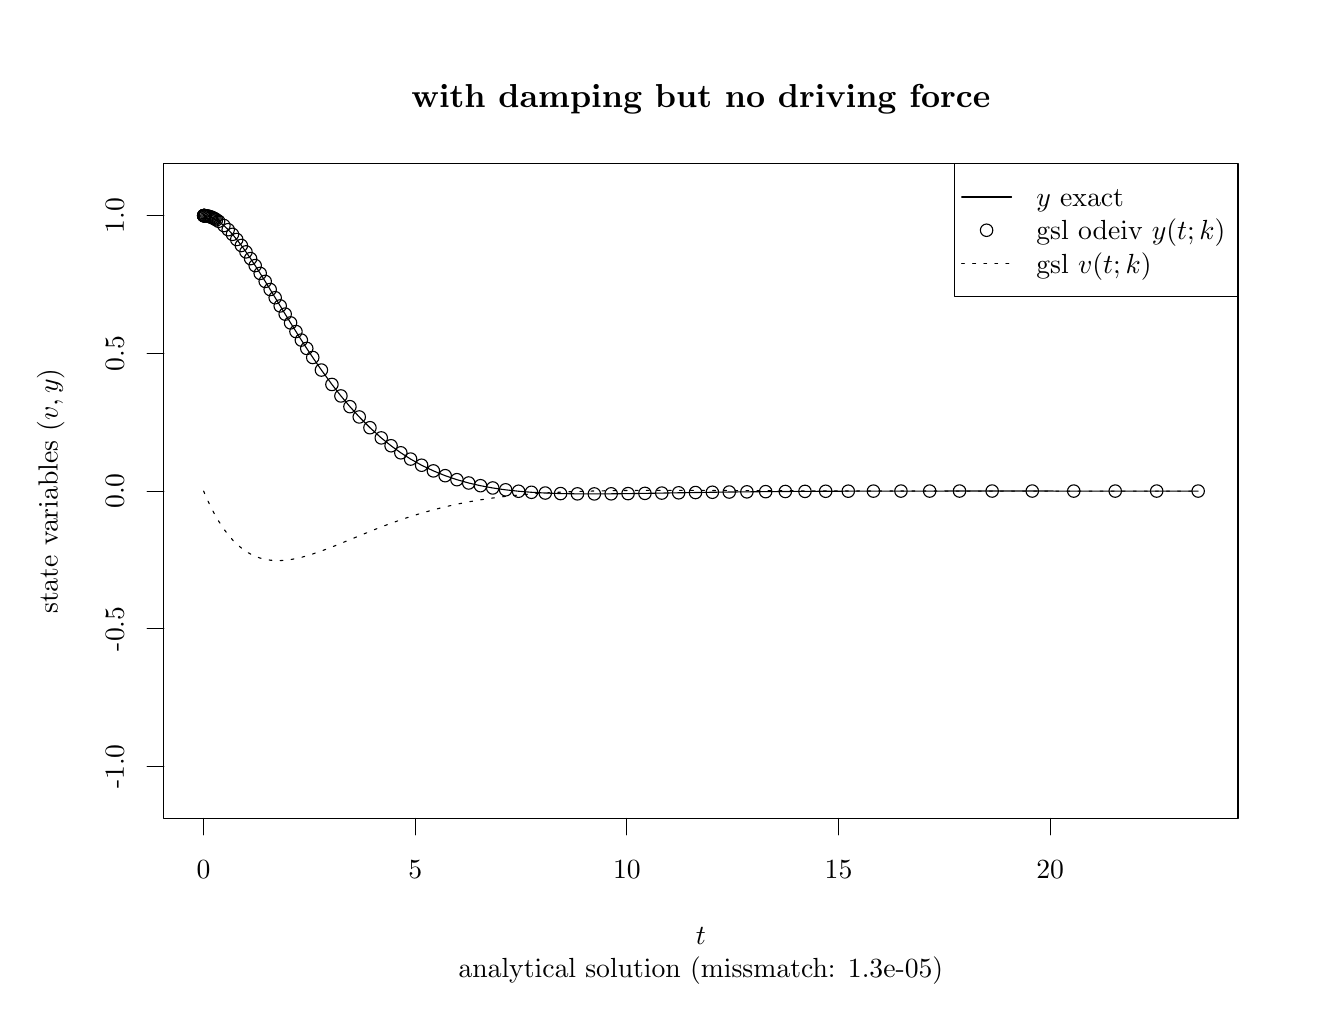
\begin{tikzpicture}[x=1pt,y=1pt]
\definecolor{fillColor}{RGB}{255,255,255}
\path[use as bounding box,fill=fillColor,fill opacity=0.00] (0,0) rectangle (462.53,346.90);
\begin{scope}
\path[clip] ( 49.20, 61.20) rectangle (437.33,297.70);
\definecolor{drawColor}{RGB}{0,0,0}

\path[draw=drawColor,line width= 0.4pt,line join=round,line cap=round] ( 63.58,278.98) --
	( 63.60,278.98) --
	( 63.63,278.98) --
	( 63.66,278.98) --
	( 63.70,278.98) --
	( 63.73,278.98) --
	( 63.76,278.98) --
	( 63.79,278.98) --
	( 63.84,278.98) --
	( 63.91,278.97) --
	( 64.04,278.97) --
	( 64.27,278.95) --
	( 64.77,278.88) --
	( 65.18,278.79) --
	( 65.60,278.68) --
	( 66.02,278.54) --
	( 66.44,278.38) --
	( 66.86,278.20) --
	( 67.28,277.99) --
	( 67.70,277.77) --
	( 68.22,277.46) --
	( 69.00,276.93) --
	( 70.92,275.39) --
	( 72.46,273.90) --
	( 74.01,272.21) --
	( 75.55,270.35) --
	( 77.22,268.19) --
	( 78.88,265.88) --
	( 80.55,263.45) --
	( 82.21,260.92) --
	( 84.02,258.10) --
	( 85.83,255.21) --
	( 87.63,252.28) --
	( 89.44,249.32) --
	( 91.25,246.35) --
	( 93.05,243.39) --
	( 95.00,240.22) --
	( 96.95,237.09) --
	( 98.89,234.02) --
	(100.84,231.00) --
	(103.01,227.72) --
	(106.14,223.18) --
	(109.94,217.98) --
	(113.19,213.82) --
	(116.45,209.94) --
	(119.81,206.23) --
	(123.68,202.34) --
	(127.77,198.65) --
	(131.31,195.81) --
	(134.84,193.27) --
	(138.37,191.01) --
	(142.35,188.78) --
	(146.61,186.74) --
	(150.86,185.01) --
	(155.11,183.56) --
	(159.37,182.36) --
	(163.62,181.39) --
	(168.05,180.57) --
	(172.71,179.89) --
	(177.38,179.39) --
	(182.04,179.01) --
	(187.03,178.74) --
	(192.57,178.55) --
	(198.66,178.44) --
	(204.76,178.42) --
	(210.85,178.46) --
	(216.94,178.53) --
	(223.04,178.62) --
	(229.13,178.72) --
	(235.23,178.83) --
	(241.32,178.92) --
	(247.41,179.02) --
	(253.51,179.10) --
	(259.89,179.17) --
	(266.67,179.24) --
	(273.77,179.30) --
	(280.87,179.34) --
	(288.35,179.38) --
	(296.52,179.41) --
	(305.61,179.43) --
	(315.56,179.45) --
	(325.94,179.45) --
	(336.72,179.46) --
	(348.51,179.46) --
	(363.00,179.46) --
	(377.99,179.45) --
	(392.98,179.45) --
	(407.96,179.45) --
	(422.95,179.45);
\end{scope}
\begin{scope}
\path[clip] (  0.00,  0.00) rectangle (462.53,346.90);
\definecolor{drawColor}{RGB}{0,0,0}

\path[draw=drawColor,line width= 0.4pt,line join=round,line cap=round] ( 63.58, 61.20) -- (369.49, 61.20);

\path[draw=drawColor,line width= 0.4pt,line join=round,line cap=round] ( 63.58, 61.20) -- ( 63.58, 55.20);

\path[draw=drawColor,line width= 0.4pt,line join=round,line cap=round] (140.06, 61.20) -- (140.06, 55.20);

\path[draw=drawColor,line width= 0.4pt,line join=round,line cap=round] (216.54, 61.20) -- (216.54, 55.20);

\path[draw=drawColor,line width= 0.4pt,line join=round,line cap=round] (293.02, 61.20) -- (293.02, 55.20);

\path[draw=drawColor,line width= 0.4pt,line join=round,line cap=round] (369.49, 61.20) -- (369.49, 55.20);

\node[text=drawColor,anchor=base,inner sep=0pt, outer sep=0pt, scale=  1.00] at ( 63.58, 39.60) {0};

\node[text=drawColor,anchor=base,inner sep=0pt, outer sep=0pt, scale=  1.00] at (140.06, 39.60) {5};

\node[text=drawColor,anchor=base,inner sep=0pt, outer sep=0pt, scale=  1.00] at (216.54, 39.60) {10};

\node[text=drawColor,anchor=base,inner sep=0pt, outer sep=0pt, scale=  1.00] at (293.02, 39.60) {15};

\node[text=drawColor,anchor=base,inner sep=0pt, outer sep=0pt, scale=  1.00] at (369.49, 39.60) {20};

\path[draw=drawColor,line width= 0.4pt,line join=round,line cap=round] ( 49.20, 79.91) -- ( 49.20,278.98);

\path[draw=drawColor,line width= 0.4pt,line join=round,line cap=round] ( 49.20, 79.91) -- ( 43.20, 79.91);

\path[draw=drawColor,line width= 0.4pt,line join=round,line cap=round] ( 49.20,129.68) -- ( 43.20,129.68);

\path[draw=drawColor,line width= 0.4pt,line join=round,line cap=round] ( 49.20,179.45) -- ( 43.20,179.45);

\path[draw=drawColor,line width= 0.4pt,line join=round,line cap=round] ( 49.20,229.22) -- ( 43.20,229.22);

\path[draw=drawColor,line width= 0.4pt,line join=round,line cap=round] ( 49.20,278.98) -- ( 43.20,278.98);

\node[text=drawColor,rotate= 90.00,anchor=base,inner sep=0pt, outer sep=0pt, scale=  1.00] at ( 34.80, 79.91) {-1.0};

\node[text=drawColor,rotate= 90.00,anchor=base,inner sep=0pt, outer sep=0pt, scale=  1.00] at ( 34.80,129.68) {-0.5};

\node[text=drawColor,rotate= 90.00,anchor=base,inner sep=0pt, outer sep=0pt, scale=  1.00] at ( 34.80,179.45) {0.0};

\node[text=drawColor,rotate= 90.00,anchor=base,inner sep=0pt, outer sep=0pt, scale=  1.00] at ( 34.80,229.22) {0.5};

\node[text=drawColor,rotate= 90.00,anchor=base,inner sep=0pt, outer sep=0pt, scale=  1.00] at ( 34.80,278.98) {1.0};

\path[draw=drawColor,line width= 0.4pt,line join=round,line cap=round] ( 49.20, 61.20) --
	(437.33, 61.20) --
	(437.33,297.70) --
	( 49.20,297.70) --
	( 49.20, 61.20);
\end{scope}
\begin{scope}
\path[clip] (  0.00,  0.00) rectangle (462.53,346.90);
\definecolor{drawColor}{RGB}{0,0,0}

\node[text=drawColor,anchor=base,inner sep=0pt, outer sep=0pt, scale=  1.20] at (243.26,318.16) {\bfseries  with damping but no driving force};

\node[text=drawColor,anchor=base,inner sep=0pt, outer sep=0pt, scale=  1.00] at (243.26,  3.60) {analytical solution (missmatch: 1.3e-05)};

\node[text=drawColor,anchor=base,inner sep=0pt, outer sep=0pt, scale=  1.00] at (243.26, 15.60) {$t$};

\node[text=drawColor,rotate= 90.00,anchor=base,inner sep=0pt, outer sep=0pt, scale=  1.00] at ( 10.80,179.45) {state variables $(v,y)$};
\end{scope}
\begin{scope}
\path[clip] ( 49.20, 61.20) rectangle (437.33,297.70);
\definecolor{drawColor}{RGB}{0,0,0}

\path[draw=drawColor,line width= 0.4pt,line join=round,line cap=round] ( 63.58,278.98) circle (  2.25);

\path[draw=drawColor,line width= 0.4pt,line join=round,line cap=round] ( 63.60,278.98) circle (  2.25);

\path[draw=drawColor,line width= 0.4pt,line join=round,line cap=round] ( 63.63,278.98) circle (  2.25);

\path[draw=drawColor,line width= 0.4pt,line join=round,line cap=round] ( 63.66,278.98) circle (  2.25);

\path[draw=drawColor,line width= 0.4pt,line join=round,line cap=round] ( 63.70,278.98) circle (  2.25);

\path[draw=drawColor,line width= 0.4pt,line join=round,line cap=round] ( 63.73,278.98) circle (  2.25);

\path[draw=drawColor,line width= 0.4pt,line join=round,line cap=round] ( 63.76,278.98) circle (  2.25);

\path[draw=drawColor,line width= 0.4pt,line join=round,line cap=round] ( 63.79,278.98) circle (  2.25);

\path[draw=drawColor,line width= 0.4pt,line join=round,line cap=round] ( 63.84,278.98) circle (  2.25);

\path[draw=drawColor,line width= 0.4pt,line join=round,line cap=round] ( 63.91,278.97) circle (  2.25);

\path[draw=drawColor,line width= 0.4pt,line join=round,line cap=round] ( 64.04,278.97) circle (  2.25);

\path[draw=drawColor,line width= 0.4pt,line join=round,line cap=round] ( 64.27,278.95) circle (  2.25);

\path[draw=drawColor,line width= 0.4pt,line join=round,line cap=round] ( 64.77,278.87) circle (  2.25);

\path[draw=drawColor,line width= 0.4pt,line join=round,line cap=round] ( 65.18,278.79) circle (  2.25);

\path[draw=drawColor,line width= 0.4pt,line join=round,line cap=round] ( 65.60,278.68) circle (  2.25);

\path[draw=drawColor,line width= 0.4pt,line join=round,line cap=round] ( 66.02,278.54) circle (  2.25);

\path[draw=drawColor,line width= 0.4pt,line join=round,line cap=round] ( 66.44,278.38) circle (  2.25);

\path[draw=drawColor,line width= 0.4pt,line join=round,line cap=round] ( 66.86,278.20) circle (  2.25);

\path[draw=drawColor,line width= 0.4pt,line join=round,line cap=round] ( 67.28,278.00) circle (  2.25);

\path[draw=drawColor,line width= 0.4pt,line join=round,line cap=round] ( 67.70,277.77) circle (  2.25);

\path[draw=drawColor,line width= 0.4pt,line join=round,line cap=round] ( 68.22,277.46) circle (  2.25);

\path[draw=drawColor,line width= 0.4pt,line join=round,line cap=round] ( 69.00,276.94) circle (  2.25);

\path[draw=drawColor,line width= 0.4pt,line join=round,line cap=round] ( 70.92,275.39) circle (  2.25);

\path[draw=drawColor,line width= 0.4pt,line join=round,line cap=round] ( 72.46,273.90) circle (  2.25);

\path[draw=drawColor,line width= 0.4pt,line join=round,line cap=round] ( 74.01,272.21) circle (  2.25);

\path[draw=drawColor,line width= 0.4pt,line join=round,line cap=round] ( 75.55,270.35) circle (  2.25);

\path[draw=drawColor,line width= 0.4pt,line join=round,line cap=round] ( 77.22,268.19) circle (  2.25);

\path[draw=drawColor,line width= 0.4pt,line join=round,line cap=round] ( 78.88,265.88) circle (  2.25);

\path[draw=drawColor,line width= 0.4pt,line join=round,line cap=round] ( 80.55,263.45) circle (  2.25);

\path[draw=drawColor,line width= 0.4pt,line join=round,line cap=round] ( 82.21,260.92) circle (  2.25);

\path[draw=drawColor,line width= 0.4pt,line join=round,line cap=round] ( 84.02,258.10) circle (  2.25);

\path[draw=drawColor,line width= 0.4pt,line join=round,line cap=round] ( 85.83,255.21) circle (  2.25);

\path[draw=drawColor,line width= 0.4pt,line join=round,line cap=round] ( 87.63,252.28) circle (  2.25);

\path[draw=drawColor,line width= 0.4pt,line join=round,line cap=round] ( 89.44,249.32) circle (  2.25);

\path[draw=drawColor,line width= 0.4pt,line join=round,line cap=round] ( 91.25,246.35) circle (  2.25);

\path[draw=drawColor,line width= 0.4pt,line join=round,line cap=round] ( 93.05,243.39) circle (  2.25);

\path[draw=drawColor,line width= 0.4pt,line join=round,line cap=round] ( 95.00,240.22) circle (  2.25);

\path[draw=drawColor,line width= 0.4pt,line join=round,line cap=round] ( 96.95,237.09) circle (  2.25);

\path[draw=drawColor,line width= 0.4pt,line join=round,line cap=round] ( 98.89,234.01) circle (  2.25);

\path[draw=drawColor,line width= 0.4pt,line join=round,line cap=round] (100.84,231.00) circle (  2.25);

\path[draw=drawColor,line width= 0.4pt,line join=round,line cap=round] (103.01,227.72) circle (  2.25);

\path[draw=drawColor,line width= 0.4pt,line join=round,line cap=round] (106.14,223.18) circle (  2.25);

\path[draw=drawColor,line width= 0.4pt,line join=round,line cap=round] (109.94,217.97) circle (  2.25);

\path[draw=drawColor,line width= 0.4pt,line join=round,line cap=round] (113.19,213.82) circle (  2.25);

\path[draw=drawColor,line width= 0.4pt,line join=round,line cap=round] (116.45,209.94) circle (  2.25);

\path[draw=drawColor,line width= 0.4pt,line join=round,line cap=round] (119.81,206.23) circle (  2.25);

\path[draw=drawColor,line width= 0.4pt,line join=round,line cap=round] (123.68,202.34) circle (  2.25);

\path[draw=drawColor,line width= 0.4pt,line join=round,line cap=round] (127.77,198.66) circle (  2.25);

\path[draw=drawColor,line width= 0.4pt,line join=round,line cap=round] (131.31,195.82) circle (  2.25);

\path[draw=drawColor,line width= 0.4pt,line join=round,line cap=round] (134.84,193.27) circle (  2.25);

\path[draw=drawColor,line width= 0.4pt,line join=round,line cap=round] (138.37,191.01) circle (  2.25);

\path[draw=drawColor,line width= 0.4pt,line join=round,line cap=round] (142.35,188.79) circle (  2.25);

\path[draw=drawColor,line width= 0.4pt,line join=round,line cap=round] (146.61,186.74) circle (  2.25);

\path[draw=drawColor,line width= 0.4pt,line join=round,line cap=round] (150.86,185.01) circle (  2.25);

\path[draw=drawColor,line width= 0.4pt,line join=round,line cap=round] (155.11,183.56) circle (  2.25);

\path[draw=drawColor,line width= 0.4pt,line join=round,line cap=round] (159.37,182.37) circle (  2.25);

\path[draw=drawColor,line width= 0.4pt,line join=round,line cap=round] (163.62,181.39) circle (  2.25);

\path[draw=drawColor,line width= 0.4pt,line join=round,line cap=round] (168.05,180.57) circle (  2.25);

\path[draw=drawColor,line width= 0.4pt,line join=round,line cap=round] (172.71,179.90) circle (  2.25);

\path[draw=drawColor,line width= 0.4pt,line join=round,line cap=round] (177.38,179.39) circle (  2.25);

\path[draw=drawColor,line width= 0.4pt,line join=round,line cap=round] (182.04,179.01) circle (  2.25);

\path[draw=drawColor,line width= 0.4pt,line join=round,line cap=round] (187.03,178.74) circle (  2.25);

\path[draw=drawColor,line width= 0.4pt,line join=round,line cap=round] (192.57,178.54) circle (  2.25);

\path[draw=drawColor,line width= 0.4pt,line join=round,line cap=round] (198.66,178.44) circle (  2.25);

\path[draw=drawColor,line width= 0.4pt,line join=round,line cap=round] (204.76,178.42) circle (  2.25);

\path[draw=drawColor,line width= 0.4pt,line join=round,line cap=round] (210.85,178.46) circle (  2.25);

\path[draw=drawColor,line width= 0.4pt,line join=round,line cap=round] (216.94,178.53) circle (  2.25);

\path[draw=drawColor,line width= 0.4pt,line join=round,line cap=round] (223.04,178.62) circle (  2.25);

\path[draw=drawColor,line width= 0.4pt,line join=round,line cap=round] (229.13,178.72) circle (  2.25);

\path[draw=drawColor,line width= 0.4pt,line join=round,line cap=round] (235.23,178.82) circle (  2.25);

\path[draw=drawColor,line width= 0.4pt,line join=round,line cap=round] (241.32,178.92) circle (  2.25);

\path[draw=drawColor,line width= 0.4pt,line join=round,line cap=round] (247.41,179.02) circle (  2.25);

\path[draw=drawColor,line width= 0.4pt,line join=round,line cap=round] (253.51,179.10) circle (  2.25);

\path[draw=drawColor,line width= 0.4pt,line join=round,line cap=round] (259.89,179.17) circle (  2.25);

\path[draw=drawColor,line width= 0.4pt,line join=round,line cap=round] (266.67,179.24) circle (  2.25);

\path[draw=drawColor,line width= 0.4pt,line join=round,line cap=round] (273.77,179.30) circle (  2.25);

\path[draw=drawColor,line width= 0.4pt,line join=round,line cap=round] (280.87,179.34) circle (  2.25);

\path[draw=drawColor,line width= 0.4pt,line join=round,line cap=round] (288.35,179.38) circle (  2.25);

\path[draw=drawColor,line width= 0.4pt,line join=round,line cap=round] (296.52,179.41) circle (  2.25);

\path[draw=drawColor,line width= 0.4pt,line join=round,line cap=round] (305.61,179.43) circle (  2.25);

\path[draw=drawColor,line width= 0.4pt,line join=round,line cap=round] (315.56,179.45) circle (  2.25);

\path[draw=drawColor,line width= 0.4pt,line join=round,line cap=round] (325.94,179.45) circle (  2.25);

\path[draw=drawColor,line width= 0.4pt,line join=round,line cap=round] (336.72,179.46) circle (  2.25);

\path[draw=drawColor,line width= 0.4pt,line join=round,line cap=round] (348.51,179.46) circle (  2.25);

\path[draw=drawColor,line width= 0.4pt,line join=round,line cap=round] (363.00,179.46) circle (  2.25);

\path[draw=drawColor,line width= 0.4pt,line join=round,line cap=round] (377.99,179.45) circle (  2.25);

\path[draw=drawColor,line width= 0.4pt,line join=round,line cap=round] (392.98,179.45) circle (  2.25);

\path[draw=drawColor,line width= 0.4pt,line join=round,line cap=round] (407.96,179.45) circle (  2.25);

\path[draw=drawColor,line width= 0.4pt,line join=round,line cap=round] (422.95,179.45) circle (  2.25);

\path[draw=drawColor,line width= 0.4pt,dash pattern=on 1pt off 3pt ,line join=round,line cap=round] ( 63.58,179.45) --
	( 63.60,179.39) --
	( 63.63,179.32) --
	( 63.66,179.24) --
	( 63.70,179.16) --
	( 63.73,179.09) --
	( 63.76,179.01) --
	( 63.79,178.93) --
	( 63.84,178.83) --
	( 63.91,178.65) --
	( 64.04,178.36) --
	( 64.27,177.83) --
	( 64.77,176.71) --
	( 65.18,175.79) --
	( 65.60,174.91) --
	( 66.02,174.04) --
	( 66.44,173.21) --
	( 66.86,172.39) --
	( 67.28,171.60) --
	( 67.70,170.84) --
	( 68.22,169.92) --
	( 69.00,168.59) --
	( 70.92,165.68) --
	( 72.46,163.64) --
	( 74.01,161.85) --
	( 75.55,160.30) --
	( 77.22,158.87) --
	( 78.88,157.67) --
	( 80.55,156.68) --
	( 82.21,155.89) --
	( 84.02,155.23) --
	( 85.83,154.77) --
	( 87.63,154.48) --
	( 89.44,154.33) --
	( 91.25,154.33) --
	( 93.05,154.45) --
	( 95.00,154.70) --
	( 96.95,155.05) --
	( 98.89,155.51) --
	(100.84,156.04) --
	(103.01,156.71) --
	(106.14,157.79) --
	(109.94,159.24) --
	(113.19,160.55) --
	(116.45,161.89) --
	(119.81,163.28) --
	(123.68,164.86) --
	(127.77,166.48) --
	(131.31,167.81) --
	(134.84,169.07) --
	(138.37,170.25) --
	(142.35,171.48) --
	(146.61,172.68) --
	(150.86,173.76) --
	(155.11,174.71) --
	(159.37,175.55) --
	(163.62,176.28) --
	(168.05,176.94) --
	(172.71,177.53) --
	(177.38,178.02) --
	(182.04,178.42) --
	(187.03,178.77) --
	(192.57,179.06) --
	(198.66,179.31) --
	(204.76,179.48) --
	(210.85,179.59) --
	(216.94,179.66) --
	(223.04,179.69) --
	(229.13,179.71) --
	(235.23,179.70) --
	(241.32,179.69) --
	(247.41,179.67) --
	(253.51,179.64) --
	(259.89,179.61) --
	(266.67,179.59) --
	(273.77,179.56) --
	(280.87,179.53) --
	(288.35,179.51) --
	(296.52,179.49) --
	(305.61,179.48) --
	(315.56,179.46) --
	(325.94,179.46) --
	(336.72,179.45) --
	(348.51,179.45) --
	(363.00,179.45) --
	(377.99,179.45) --
	(392.98,179.45) --
	(407.96,179.45) --
	(422.95,179.45);
\definecolor{fillColor}{RGB}{255,255,255}

\path[draw=drawColor,line width= 0.4pt,line join=round,line cap=round,fill=fillColor] (334.80,297.70) rectangle (437.33,249.70);

\path[draw=drawColor,line width= 0.4pt,line join=round,line cap=round] (337.50,285.70) -- (355.50,285.70);

\path[draw=drawColor,line width= 0.4pt,dash pattern=on 1pt off 3pt ,line join=round,line cap=round] (337.50,261.70) -- (355.50,261.70);

\path[draw=drawColor,line width= 0.4pt,line join=round,line cap=round] (346.50,273.70) circle (  2.25);

\node[text=drawColor,anchor=base west,inner sep=0pt, outer sep=0pt, scale=  1.00] at (364.50,282.25) {$y$ exact};

\node[text=drawColor,anchor=base west,inner sep=0pt, outer sep=0pt, scale=  1.00] at (364.50,270.25) {gsl odeiv $y(t;k)$};

\node[text=drawColor,anchor=base west,inner sep=0pt, outer sep=0pt, scale=  1.00] at (364.50,258.25) {gsl $v(t;k)$};
\end{scope}
\end{tikzpicture}
